% Chapter 1
\chapter{Introducción general} % Main chapter title

Este capitulo explica los motivos detrás de la decisión de realizar este trabajo final. Realiza una comparación entre el dispositivo desarrollado y productos de características similares que están disponibles en el mercado. Y finalmente enumera los alcances y objetivos del trabajo final.

\label{Chapter1} % For referencing the chapter elsewhere, use \ref{Chapter1} 
\label{IntroGeneral}

%----------------------------------------------------------------------------------------

% Define some commands to keep the formatting separated from the content 
\newcommand{\keyword}[1]{\textbf{#1}}
\newcommand{\tabhead}[1]{\textbf{#1}}
\newcommand{\code}[1]{\texttt{#1}}
\newcommand{\file}[1]{\texttt{\bfseries#1}}
\newcommand{\option}[1]{\texttt{\itshape#1}}
\newcommand{\grados}{$^{\circ}$}

%----------------------------------------------------------------------------------------

%\section{Introducción}

%----------------------------------------------------------------------------------------
\section{Motivación}

Desde el año 1991 en adelante, todos los fabricantes de vehículos de combustión interna están obligados a incluir en sus vehículos un sistema electrónico de diagnóstico. Este sistema, conocido por sus siglas en inglés como OBD (On-Board Diagnostics), realiza las tareas de muestrear sensores que están conectados físicamente sobre el motor y alertar al conductor, a través de un indicador en el tablero, cuando el motor no está funcionando dentro de los parámetros de operación. También mantiene un registro interno de los fallos ocurridos durante la vida del mismo, para luego ser descargado por el mecánico encargado de realizar tareas de reparación o puesta a punto, y así facilitar su trabajo.
Actualmente existen grupos de entusiastas y coleccionistas que poseen vehículos fabricados antes de que el sistema OBD se haga obligatorio. Y por esa razón, no tienen la posibilidad de hacer un monitoreo del funcionamiento del motor de su vehículo. Tampoco es posible mantener un registro de si hubo eventos de fallas o momentos de operación fuera de rango, información útil para su mantenimiento preventivo.
Por esto es que se tomó la decisión de desarrollar para este Trabajo Final, un dispositivo que cumpla las mismas funciones que un OBD, pero para vehículos antiguos que no tienen instalado dicho sistema de fábrica.

\section{Alcance y objetivos}

El objetivo de este trabajo final fue de desarrollar un prototipo que realizara las funciones de muestrear, guardar y mostrar en tiempo real, los datos adquiridos por los sensores del motor. 

\section{Estado del arte}

Actualmente en el mercado existen productos de características y funcionalidades similares. Para poder hacer una comparación, se eligieron los productos de entrada de dos marcas distintas. Uno es el Fueltech-FT300, que puede verse en la figura \ref{fig:comparativa} \subref{fig:fueltech},  y el otro es el HT-193000 de Halltech, visto en la figura \ref{fig:comparativa}\subref{fig:halltech}. La tabla \ref{tab:comparativa} hace una comparativa entre estos productos y el dispositivo desarrollado para el Trabajo Final, enlistando sus funcionalidades y características. Cabe destacar que al momento de escribir esta memoria, no existen un producto de estas características que esté diseñado o fabricado en Argentina.

\begin{figure}[htpb]
\centering
\begin{subfigure}{.4\textwidth}
\centering
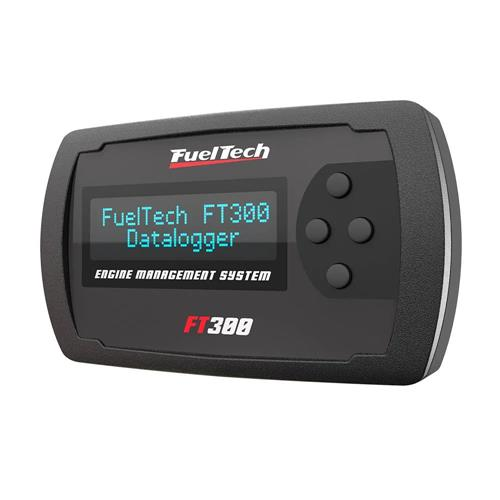
\includegraphics[width=\textwidth]{./Figures/fueltech-ft300.jpg}
\caption{Fueltech FT-300}
\label{fig:fueltech}
\end{subfigure}
\hfill
\begin{subfigure}{.5\textwidth}
\centering
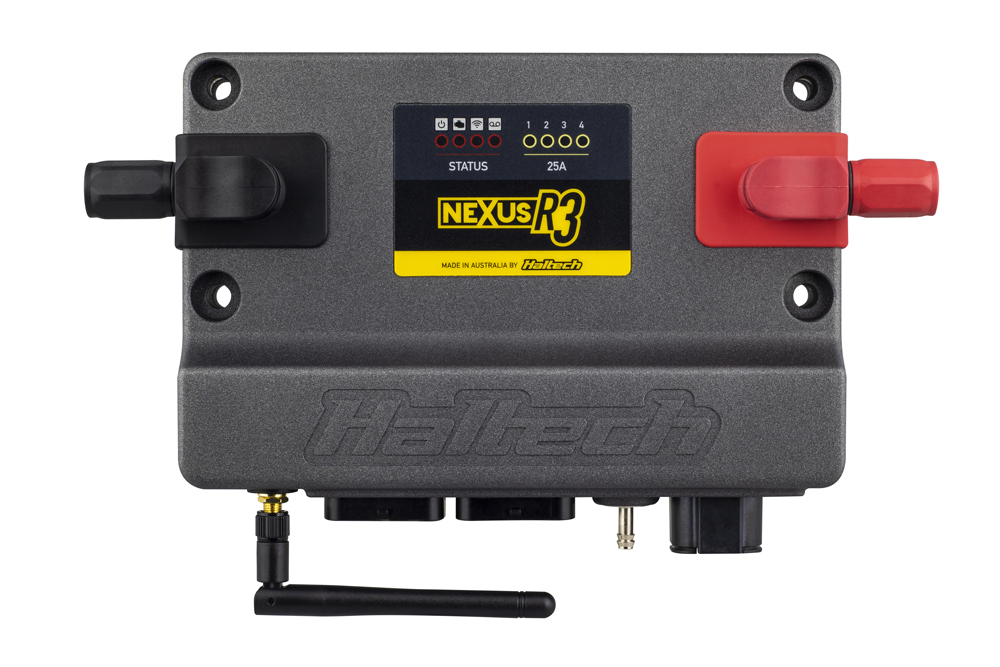
\includegraphics[width=\textwidth]{./Figures/HT-193000_00.JPG}
\caption{Halltech HT-193000}
\label{fig:halltech}
\end{subfigure}
\hfill
\caption{Fotografias de ambas ECUs, a la izquierda (A) se ve la ECU FT-300 de Fueltech, y a la derecha (B) se ve la ECU HT-193000 de Halltech.}
\label{fig:comparativa}
\end{figure}

\vspace{25px}

\begin{table}[h]
	\centering
	\caption[caption corto]{Tabla comparativa entre dispositivos}
	\begin{tabular}{l c c c}    
		\toprule
		\textbf{ }     & \textbf{Halltech HT-193000} & \textbf{Fueltech-300} & \textbf{Trabajo Final}\\
		\midrule
		Entradas temp.			&  0 &   2 &  3\\
		Presión de aceite		& Si &  Si & Si\\
		Presión de combustible	& Si &  Si & No\\
		Presión de admisión		& Si &  Si & No\\
		Sonda Lambda			& Si &  Si & Si\\
		R.P.M.					& Si &  Si & Si\\
		Entradas analógicas		& 11 &  0  &  0\\
		Control de inyección	& Si &  Si & No\\
		\bottomrule
		\hline
	\end{tabular}
	\label{tab:comparativa}
\end{table}


